\mysection{Division du Travail}\label{Div_Trav}

On souhaite que le produit final de ce travail soit un jeu de Morpion déployé dans le robot KUKA youBot et commande par une interface graphique, comme on a déjà décrit ci-dessus. 

Sur base de ces objectifs, on peut séparer le travail en deux phases différentes que seront développés de manière séquentielle:
\begin{itemize}
	\item Phase 1: à propos du système robotique dans un environnement de simulation, lequel on doit traiter et solutionner les problèmes de commande du système;
	\item Phase 2: à propos de la mise en oeuvre du jeu en environnement physique, lequel on doit construire les différentes interfaces du système: robot $ \leftrightarrow $ PC et PC $ \leftrightarrow $ utilisateur.
\end{itemize}


Les actions et les sous-produits de la première phase du projet seront séparés en deux structures et développés en parallèle: une concernant l’étude et génération de la trajectoire exécuté par l’effecteur du robot (structure A) et l’autre concernant l’étude et mise en oeuvre de l’asservissement de l’effecteur (structure B).

Après la conclusion de chaque structure, on doit faire l’intégration des parties qui ont déjà été développés. Ainsi, on prévoit observer dans l’environnement de simulation Matlab l’effectuer réaliser une trajectoire stipulée. 

De la même manière, la deuxième phase sera séparé en deux structures: une concernant la communication du robot avec l’ordinateur (structure A) et l’autre concernant la création de l’interface graphique de communication de l’ordinateur avec l’utilisateur (structure B).

De la répartition du projet en deux phases bien définies, on a pu séparer le projet en deux différentes domaines: d’automatique et d’informatique. Ainsi, lorsqu'on complète la première phase à propos de la problématique de contrôle, on aura déjà obtenu résultats bien satisfaisantes référents les objectifs d'apprentissage de ce projet.
Le diagramme en arbre suivant décrit les différentes phases et structures qu’on a réparti le projet:


\begin{figure}[H]
	\begin{center}	
		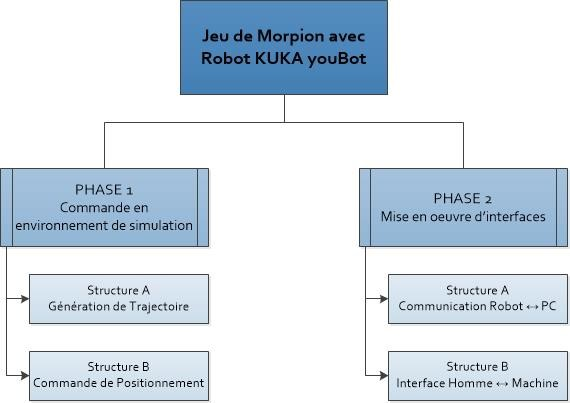
\includegraphics[width=8cm]{./diagram.jpg}
		\caption{Diagramme en arbre de la structure de découpage du projet }
		\label{fig:diagram}
	\end{center}
\end{figure}
\newpage

\mysubsection{Définition des tâches à entreprendre}

Ci-dessous, on a défini les tâches à entreprendre en chaque structure de découpage du projet. Dans la section \ref{Methodologie} on a décrit les tâches de façon plus détaillée.
